\documentclass[a4paper, 11pt, oneside]{memoir}
\semiisopage
\usepackage[es]{config/ifcommands}


%%%%%%%%%%
% ESTILO %
%%%%%%%%%%

%=========================================================================================================%
% default, bianchi, bringhurst, brotherton, chappell, crosshead, culver, dash, demo2, demo3, dowding, ell,%
% ger, komalike, lyhne, madsen, ntglike, pedersen, southall, tandh, thatcher, veelo, verville, wilsondob  %
%=========================================================================================================%

% \chapterstyle{ger} -> Entre lineas todo
\chapterstyle{madsen}
% \chapterstyle{veelo} -> El que venía, chulo
% \chapterstyle{verville} -> Simple, centrado

\pdfobjcompresslevel 0
\raggedbottom

%%%%%%%%%%%%%%%
% INTOFMACIÓN %
%%%%%%%%%%%%%%%

\newcommand{\egilea}{Jon Ortega Goikoetxea}
\newcommand{\zuzendariak}{Miren Bermejo Llopis}
\newcommand{\izenburua}{Desarrollo de una Plataforma Web Interactiva de Datos Musicales Obtenidos de la API de Spotify}
\newcommand{\data}{\today}
\newcommand{\ikasketak}{Grado en Ingeniería Informática}
\newcommand{\espezialitatea}{Ingeniería de Software}

\newcommand{\castellano}

\input config/macros

\title{\izenburua}
\author{\egilea}
\date{\data}

%=====================================================================%

\begin{document}

%%%%%%%%%%%
% PORTADA %
%%%%%%%%%%%

%% SI HAY UNA PORTADA ESPECIAL (EN PDF), DESCOMENTAR%%
% 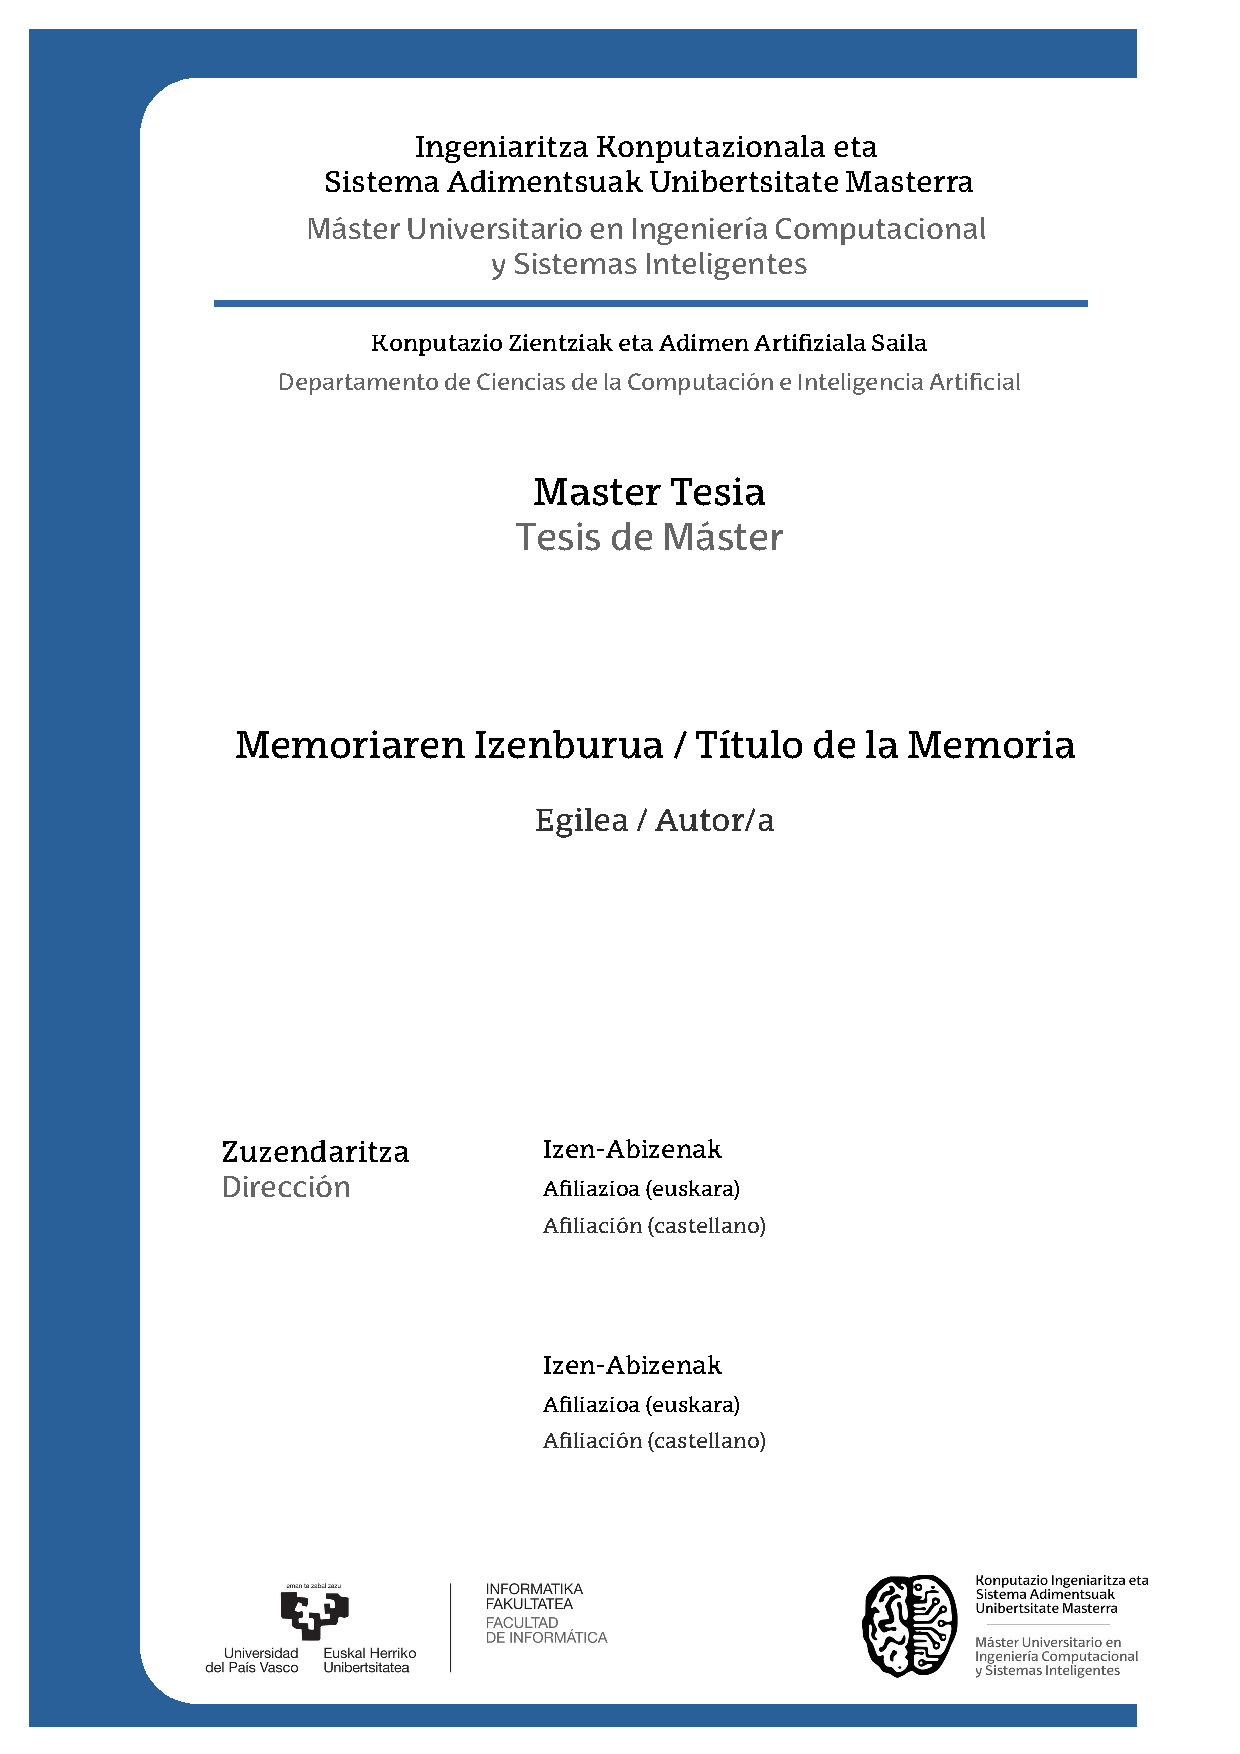
\includepdf[pages={1-}]{content/cover/cover.pdf}
% \cleardoublepage
%% EN CASO DE NO TENER UNA PORTADA ESPECIAL, DESCOMENTAR %%
\input content/cover/cover_informatika

\cleardoublepage
\frontmatter

%%%%%%%%%%%%%%%%%%%
% AGRADECIMIENTOS %
%%%%%%%%%%%%%%%%%%%

\chapter*{Agradecimientos}
\input content/chapters/agradecimientos
\cleardoublepage

%%%%%%%%%%%
% RESUMEN %
%%%%%%%%%%%

\chapter*{Resumen}
\input content/chapters/resumen
\cleardoublepage

%%%%%%%%%%%
% ÍNDICES %
%%%%%%%%%%%

\tableofcontents
\clearpage
\listoffigures
\clearpage
\listoftables
\clearpage
% \listofalgorithms
% \addcontentsline{toc}{chapter}{Índice de algoritmos}

%%%%%%%%%%%%%
% CONTENIDO %
%%%%%%%%%%%%%

\cleardoublepage
\mainmatter
\pagestyle{ruled}

\chapter{Introducción} \label{ch:introduccion}
\input content/chapters/1_introduccion
\cleardoublepage

\chapter{Estado del Arte} \label{ch:estadoDelArte}
\input content/chapters/2_estadoDelArte
\cleardoublepage

\chapter{Planificación} \label{ch:planificacion}
\input content/chapters/2_planificacion
\cleardoublepage

\chapter{Análisis} \label{ch:analisis}
\input content/chapters/3_analisis
\cleardoublepage

\chapter{Diseño} \label{ch:diseño}
\input content/chapters/4_diseno
\cleardoublepage

\chapter{Implementación} \label{ch:implementacion}
\input content/chapters/5_implementacion
\cleardoublepage

\chapter{Pruebas} \label{ch:pruebas}
\input content/chapters/6_pruebas
\cleardoublepage

\chapter{Despliegue} \label{ch:despliegue}
\input content/chapters/7_despliegue
\cleardoublepage

\chapter{Conclusiones} \label{ch:conclusiones}
\input content/chapters/8_conclusiones
\cleardoublepage

%%%%%%%%%%%%%
% APÉNDICES %
%%%%%%%%%%%%%

\backmatter
\appendix

\chapter{Apéndice} \label{ch:apendice}
\input content/chapters/appendix

%%%%%%%%%%%%%%%%
% BIBLIOGRAFIA %
%%%%%%%%%%%%%%%%

\bibliographystyle{IEEEtran}
\bibliography{referencias}
%% ALDATU HEMEN EDUKIEN ZERRENDAN AGERTUKO DENA 
\addcontentsline{tof}{chapter}{\bibname}

\end{document}
